\section{Coalition Building}\label{sec:coalition}
Coalition building is a crucial process having direct impact on the quality of the analytics results. Figure~\ref{fig:smet} shows how data lineage is impacted by the processing lineage and in particular by i) the \textit{coalition a\-greement} $\textit{CA}_C$ (i.e., the CA-driven transformations adopted for a give coalition) and by ii) the transformation produced by the different jobs (job-specific transformation) part of a given coalition \coalition{}.
Let us consider job $\job{1}^{\org{1}}$ of Figure~\ref{fig:smet} it receives as input the data \trans{1}(\dataset{1}) based on the dataset obtained by \dataset{1} after the transformation  \trans{1} which is associated to the data lineage by our AC model. It then produce a data that is the job-specific transformation on the input data (i.e., \trans{1}(\dataset{1})) generating \dataset{2}.
We note that our Big Data Analytics pipeline models includes alternatives allowing different processing lineage (linear independent path in the Big data graph G) doing the same analytics but using different jobs (e.g., a lineage including k-means or a lineage using c-means). This will lead to different job-specific transformation on the data for the same Big Data pipeline.
In this paper, for the sake of simplicity we i) consider different coalitions for each processing lineage, ii) coalitions made of trustworthy organizations \org{i} providing candidate services for each job and iii) job-specific transformation not influenced by the organizations' behavior.
In this scenario, since any coalition of a given processing lineage will produce the same job-specific data transformation, the analytics pipeline quality is impacted only by the \textit{coalition agreement} $\textit{CA}_C$ or rather by the transformations \trans{i} imposed by the given coalition \coalition{} on the data lineage.
In the following we first present metrics to evaluate data quality across the data lineage, and then a set of solutions to build coalitions for  given Big Data pipeline ensuring a given data quality.

%\begin{example}\label{ex:p1j}
%The choice of the specific deployment has an impact on the way in which the coalition \coalition{} of organizations \org{i} is formed as discussed in the following of this section.
%Let us consider the following example where we have a pipeline made of just one ingestion job that can be offered by service provider $s_1$ or by the service provider $s_2\] In case the $s_1$ is selected the transformation $T_1$ is triggered according to the authorization $s_1$ has on the data, in this example $s_1$ has full control meaning that transformation $t_1$ is empty. In case the $s_2$ is selected the transformation $T_2$ is triggered according to the authorization $s_2$ has on the data and in this example data labelled as PII are removed.
%\end{example}
%Considering the two data lineage generated by the two different coalition in Example\ref{ex:p1j} the one involving $s_2$ produce a significant changes to data compared to the other one. This data changes can have direct impact on the quality of the analytics outcomes, therefore our goal is to build coalitions ensuring specific data quality. This coalition building problem can be assimilated to xxx showing an exponential complexity ...
%In the following we fist introduce our data quality metrics and then our euristics to solve the problem of coalition building

%\subsection{Data Quality metrics}
%\subsection{Coalition Heuristics}
\subsection{Metrics}

Data quality is a largely studied topic for the database management research communities,
and is in general focused on the quality of the data source rather then on the quality of the data outcomes or of the data while used in the processing pipeline.
In \cite{BigDataQaulitySurvey} a survey on big data quality is proposed mentioning the well known categories of big data quality grouped by intrinsic,
contextual representational and accessibility categories.
It also presents an holistic quality management model where the importance of data quality during processing is just mentioned in terms of requirements for the pre-processing job (e.g., data enhancement due to cleaning jobs).
In this paper we depart from this idea on data quality at pre processing time only measuring it at each step of the big data pipeline.
%data quality are divided into four categories: intrinsic, contextual representational and accessibility that covers almost all the aspects of data at ingestion time


In the following we present a set of metrics to evaluate the quality of the data at each step of the big data pipeline.
We

The proposed metrics can be classified into two categories, namely quantitative and statistical.
Initially, these metrics are applied to the original dataset (X) without any transformations, and subsequently, they are applied to the transformed dataset (Y).
The quantitative approach facilitates the calculation of the amount of data that has been lost during the transformation by enumerating the differences between X and Y.
On the other hand, the statistical approach takes into consideration the changes in certain statistical properties before and after the transformation.
These metrics can be applied either to the entire dataset or specific features.
The features can be assigned either equal or varying weights, which enables the prioritization of important features that were lost during the transformation.

% \item Metrica quantitativa
% \item Mean Squared Error (MSE). Let us considera two dataset X and Y of the same size. The MSE is defined as: $MSE(X,Y) = \frac{1}{n}\sum_{i=1}^{n}(x_i - y_i)^2\]
% \item Metrica quantitativa pesata
% \item Parametri statistici (deviazione standard, media, ecc)

\subsubsection{Jaqard coefficent}
Let us consider two dataset X and Y of the same size.
The Jaqard coefficent is defined as:\[J(X,Y) = \frac{|X \cap Y|}{|X \cup Y|}\]
And is computed by dividing the cardinality of the intersection of two sets by the cardinality of their union.
It ranges from 0 to 1, where 0 indicates no similarity and 1 indicates complete similarity between the sets.

The use of Jaccard coefficient has several advantages when applied to datasets.
Unlike other similarity measures, such as Euclidean distance, Jaccard coefficient is not affected by the magnitude of the values in the dataset.
This property makes it suitable for datasets with categorical variables or nominal data, where the values do not have a meaningful numerical interpretation.

\subsubsection{Jaqard coefficent with weights} Let us consider two dataset X and Y of the same size.
The Jaqard coefficent is defined as:\[J(X,Y) = \frac{\sum_{i=1}^{n}w_i(x_i \cap y_i)}{\sum_{i=1}^{n}w_i(x_i \cup y_i)}\]
Which is computed by dividing the cardinality of the intersection of two sets by the cardinality of their union, weighted by the weights assigned to the elements in the sets.
Weights allow for the prioritization of certain features or elements in the datasets.
This approach can be particularly useful when some elements in the dataset have more importance or relevance than others.
By assigning weights to the elements, the weighted Jaccard similarity can account for this importance and provide a more accurate measure of similarity.

% \subsubsection{Kullback-Leibler divergence}
% Let us consider two dataset X and Y of the same size.
% The KL divergence is defined as:\[KL(X,Y) = \sum_{i=1}^{n}x_i \log \frac{x_i}{y_i}\]
% Which is computed by taking the sum of the product of each element in the first dataset and the logarithm of the ratio of the same element in the second dataset.
% The KL divergence is a measure of the difference between two probability distributions and is useful for comparing the dissimilarity of two datasets.


% \subsubsection{Kullback-Leibler divergence with weights} Let us consider two dataset X and Y of the same size. The weighted KL divergence is defined as:

% \[KL(X,Y) = \sum_{i=1}^{n}w_i(x_i \log \frac{x_i}{y_i})\]

% The weighted KL divergence is a variant of the KL divergence that incorporates weights to the elements in the datasets being compared.
% It allows for the prioritization of certain features or elements in the datasets.
% This approach can be particularly useful when some elements in the dataset have more importance or relevance than others.
% By assigning weights to the elements, the weighted KL divergence can account for this importance and provide a more accurate measure of dissimilarity.

\subsubsection{Jensen-Shannon Divergence}

Let us consider two datasets X and Y of the same size. The Jensen-Shannon divergence (JSD) is a symmetrized version of the KL divergence and can be used to measure the dissimilarity between the two probability distributions.

The JSD between X and Y can be calculated as follows:

\[JSD(X, Y) = \frac{1}{2} \left( KL(X || M) + KL(Y || M) \right)\]

where M = 0.5 * (X + Y) is the average distribution.

The JSD incorporates both the KL divergence from X to M and from Y to M. It provides a balanced measure of dissimilarity that is symmetric and accounts for the contribution from both datasets.

The JSD can be useful for comparing the dissimilarity of two datasets when you want a symmetric and normalized measure that considers the overall distribution of the data.

By utilizing the JSD, you can obtain a more comprehensive understanding of the dissimilarity between X and Y, taking into account the characteristics of both datasets.

\subsubsection{Jensen-Shannon Divergence with Weights}

Let us consider two datasets X and Y of the same size. The Jensen-Shannon divergence (JSD) can be extended to incorporate weights in the calculation, resulting in a weighted version of the divergence. This weighted Jensen-Shannon divergence accounts for the importance or relevance of specific features or elements in the datasets being compared.

The weighted Jensen-Shannon divergence between X and Y, denoted as JSDw(X, Y), is defined as:

\[JSDw(X, Y) = \frac{1}{2} \left( \sum_{i=1}^{n} w_i \left( x_i \log \frac{x_i}{m_i} \right) + \sum_{i=1}^{n} w_i \left( y_i \log \frac{y_i}{m_i} \right) \right)\]

where x\_i and y\_i are the elements of X and Y, respectively, w\_i represents the weights assigned to each element, and \[m_i = \frac{{x_i + y_i}}{2}\] is the average of the corresponding elements.

By incorporating weights into the JSD calculation, the weighted Jensen-Shannon divergence provides a more accurate measure of dissimilarity between X and Y, considering the importance of individual elements based on the assigned weights. This approach is particularly useful when certain elements in the datasets have varying levels of significance, enabling a more tailored analysis of dissimilarity.
\subsection{Metrica Composta tipo vikor}
?
\subsection{Metrica Composta vikor weighted (TOPSIS)}
?

\subsection{Problema}
The metrics established will enable the quantification of data loss pre- and post-transformations.
In the event of multiple service interactions, each with its respective transformation, efforts will be made to minimize the loss of information while upholding privacy and security standards.
Due to the exponential increase in complexity as the number of services and transformations grow, identifying the optimal path is inherently an NP-hard problem.
As such, we propose some heuristics to approximate the optimal path as closely as possible. To evaluate their efficacy, the heuristically generated paths will be compared against the optimal solution.
\subsection{Prova di NP-hardness}

\subsection{Euristics}
\lstset{ %
  backgroundcolor=\color{white},   % choose the background color; you must add \usepackage{color} or \usepackage{xcolor}
  basicstyle=\footnotesize,        % the size of the fonts that are used for the code
  breakatwhitespace=false,         % sets if automatic breaks should only happen at whitespace
  breaklines=true,                 % sets automatic line breaking
  captionpos=b,                    % sets the caption-position to bottom
  commentstyle=\color{commentsColor}\textit,    % comment style
  deletekeywords={list},            % if you want to delete keywords from the given language
  escapeinside={\%*}{*)},          % if you want to add LaTeX within your code
  extendedchars=true,              % lets you use non-ASCII characters; for 8-bits encodings only, does not work with UTF-8
  frame=tb,	                   	   % adds a frame around the code
  keepspaces=true,                 % keeps spaces in text, useful for keeping indentation of code (possibly needs columns=flexible)
  keywordstyle=\color{keywordsColor}\bfseries,       % keyword style
  language=Python,                 % the language of the code (can be overrided per snippet)
  otherkeywords={*,to,function, Seq, add,empty},           % if you want to add more keywords to the set
  numbers=left,                    % where to put the line-numbers; possible values are (none, left, right)
  numbersep=5pt,                   % how far the line-numbers are from the code
  numberstyle=\tiny\color{commentsColor}, % the style that is used for the line-numbers
  rulecolor=\color{black},         % if not set, the frame-color may be changed on line-breaks within not-black text (e.g. comments (green here))
  showspaces=false,                % show spaces everywhere adding particular underscores; it overrides 'showstringspaces'
  showstringspaces=false,          % underline spaces within strings only
  showtabs=false,                  % show tabs within strings adding particular underscores
  stepnumber=1,                    % the step between two line-numbers. If it's 1, each line will be numbered
  stringstyle=\color{stringColor}, % string literal style
  tabsize=2,	                   % sets default tabsize to 2 spaces
  title=\lstname,                  % show the filename of files included with \lstinputlisting; also try caption instead of title
  columns=fixed                    % Using fixed column width (for e.g. nice alignment)
}
\subsection*{Greedy}
The greedy algorithm is a heuristic that can be used to minimize the quantity of information lost by making locally optimal choices at each step in the hope of achieving a globally optimal solution.
For instance, in our service selection problem, the greedy algorithm can be used to select services in order of their information loss, starting with the service with the lowest information loss.
This strategy ensures that services with lower information loss are selected first, minimizing the overall quantity of information lost.
Pseudo-code for the greedy algorithm is presented in Algorithm 1.
\begin{lstlisting}[frame=single,caption={Greedy Heuristic Pseudocode},label={lst:greedy}]
function GreedyHeuristic(Set nodes):

  selectedNodes = empty
  while nodes is not empty:
    minMetricNode = None
    minMetricValue = infinity
    for node in nodes:
      currentMetric = calculateMetric(node)
      if currentMetric < minMetricValue:
        minMetricValue = currentMetric
        minMetricNode = node
        add minMetricNode to selectedNodes
        remove minMetricNode from nodes
  return selectedNodes
        \end{lstlisting}

The pseudocode and is made of one function, GreedyHeuristic, which takes a set of nodes as input and returns a set of selected nodes.
The function starts by initializing an empty set of selected nodes.
Then, while there are still nodes to be selected, the algorithm iterates over the nodes and selects the node with the lowest metric value.
The selected node is then added to the set of selected nodes and removed from the set of nodes.
Finally, the set of selected nodes is returned.

\subsection*{Sliding Window}



The sliding window algorithm is a heuristic that can be used to minimize the quantity of information lost by considering a subset of the available services defined by a fixed or moving window.
For example, in our service selection problem where the quantity of information lost needs to be minimized, the sliding window algorithm can be used to select services composition that have the lowest information loss within a fixed-size window.
This strategy ensures that only services with low information loss are selected, minimizing the overall quantity of information lost.
Pseudo-code for the sliding window algorithm is presented in Algorithm 2.
\begin{lstlisting}[frame=single, caption={Sliding Window Heuristic} ,label={lst:slidingwindow}]
function SlidingWindowHeuristic(Seq sequence, int windowSize):

  selectedNodes = empty
  for i from 0 to length(sequence) - windowSize:
    minMetricNode = None
    minMetricValue = infinity
    for j from i to i + windowSize:
      currentMetric = calculateMetric(sequence[j])
      if currentMetric < minMetricValue:
        minMetricValue = currentMetric
        minMetricNode = sequence[j]
    add minMetricNode to selectedNodes
  return selectedNodes
\end{lstlisting}
The pseudocode is made of one function, SlidingWindowHeuristic, which takes a sequence of nodes and a window size as input and returns a set of selected nodes.
The function starts by initializing an empty set of selected nodes.
Then, for each node in the sequence, the algorithm iterates over the nodes in the window and selects the node with the lowest metric value.
The selected node is then added to the set of selected nodes.
Finally, the set of selected nodes is returned.


The utilization of heuristics in service selection can be enhanced through the incorporation of techniques derived from other algorithms, such as Ant Colony Optimization or Tabu Search.
By integrating these approaches, it becomes feasible to achieve a more effective and efficient selection of services, with a specific focus on eliminating paths that have previously been deemed unfavorable.

\usetikzlibrary{positioning}
\usetikzlibrary{backgrounds}
\begin{figure}
  \centering
  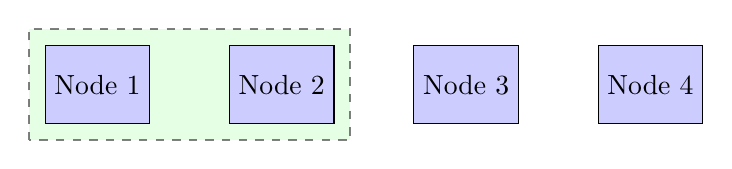
\begin{tikzpicture}

    % Nodes
    \node[rectangle, draw, minimum width=1cm, minimum height=1cm, fill=blue!20] (node1) {Node 1};
    \node[rectangle, draw, minimum width=1cm, minimum height=1cm, fill=blue!20, right=of node1] (node2) {Node 2};
    \node[rectangle, draw, minimum width=1cm, minimum height=1cm, fill=blue!20, right=of node2] (node3) {Node 3};
    \node[rectangle, draw, minimum width=1cm, minimum height=1cm, fill=blue!20, right=of node3] (node4) {Node 4};

    % Windows
    \begin{scope}[on background layer]
      \draw[thick, dashed, fill=green!20, opacity=0.5] ([shift={(-0.2,-0.2)}]node1.south west) rectangle ([shift={(0.2,0.2)}]node2.north east);
    \end{scope}

  \end{tikzpicture}

  \vspace{5pt}

  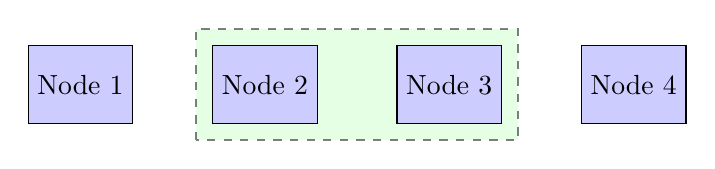
\begin{tikzpicture}

    % Nodes
    \node[rectangle, draw, minimum width=1cm, minimum height=1cm, fill=blue!20] (node1) {Node 1};
    \node[rectangle, draw, minimum width=1cm, minimum height=1cm, fill=blue!20, right=of node1] (node2) {Node 2};
    \node[rectangle, draw, minimum width=1cm, minimum height=1cm, fill=blue!20, right=of node2] (node3) {Node 3};
    \node[rectangle, draw, minimum width=1cm, minimum height=1cm, fill=blue!20, right=of node3] (node4) {Node 4};

    % Windows
    \begin{scope}[on background layer]
      \draw[thick, dashed, fill=green!20, opacity=0.5] ([shift={(-0.2,-0.2)}]node2.south west) rectangle ([shift={(0.2,0.2)}]node3.north east);
    \end{scope}


  \end{tikzpicture}

  \vspace{5pt}


  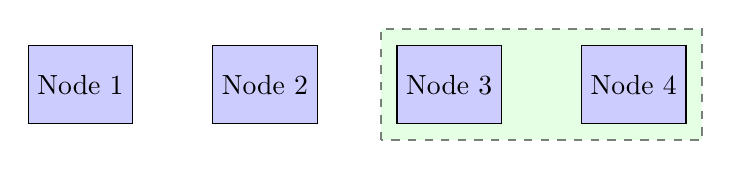
\begin{tikzpicture}

    % Nodes
    \node[rectangle, draw, minimum width=1cm, minimum height=1cm, fill=blue!20] (node1) {Node 1};
    \node[rectangle, draw, minimum width=1cm, minimum height=1cm, fill=blue!20, right=of node1] (node2) {Node 2};
    \node[rectangle, draw, minimum width=1cm, minimum height=1cm, fill=blue!20, right=of node2] (node3) {Node 3};
    \node[rectangle, draw, minimum width=1cm, minimum height=1cm, fill=blue!20, right=of node3] (node4) {Node 4};

    % Windows
    \begin{scope}[on background layer]
      \draw[thick, dashed, fill=green!20, opacity=0.5] ([shift={(-0.2,-0.2)}]node3.south west) rectangle ([shift={(0.2,0.2)}]node4.north east);
    \end{scope}
  \end{tikzpicture}

  \caption{Sliding Window Heuristic}
  \label{fig:slidingwindow}
\end{figure}